{\color{gray}\hrule}
\begin{center}
\section{Setting up the simulation}
\textbf{Processing SELECT and STASIS trial data, and fitting unknown parameters to our model}
\bigskip
\end{center}
{\color{gray}\hrule}

\subsection{Data Measured in Trials}
To accurately model weight loss across different BMI categories, we analyzed data from both the SELECT and STASIS trials \cite{Ryan2024}. Our goal was to determine the true treatment effect of semaglutide assuming perfect adherence.

\begin{table}[h]
\centering
\begin{tabular}{|l|c|c|c|}
\hline
\textbf{Parameter} & \textbf{SELECT Trial} & \textbf{STASIS Trial} & \textbf{Units} \\
\hline
Duration & 4 years & 2 years & years \\
Baseline Weight & 105.6 & BMI dependent & kg \\
Baseline Glucose & 95.4 & BMI dependent & mg/dl \\
Baseline Insulin & 12.6 & BMI dependent & $\mu$U/ml \\
Height & 1.65 & 1.8 & m \\
Age & 47.3 & 30 & years \\
\hline
\end{tabular}
\caption{Key measurements from both trials at baseline}
\end{table}

For the SELECT trial, we incorporated three key components:
\begin{itemize}
    \item Estimated Treatment Differences (ETD) for each BMI category
    \item Placebo group weight loss (-1.5\% at 4 years)
    \item Adherence adjustment (+1.5\% based on first on-treatment analysis)
\end{itemize}

The adherence-adjusted weight loss was calculated using:
\begin{equation}
    \text{Adjusted Weight Loss} = (\text{ETD} + \text{Placebo Loss}) + 1.5\%
\end{equation}

\begin{table}[h]
\centering
\begin{tabular}{|l|c|c|c|c|}
\hline
\textbf{BMI Group} & \textbf{ETD (\%)} & \textbf{Placebo (\%)} & \textbf{Initial (\%)} & \textbf{Adjusted (\%)} \\
\hline
BMI $<$30 & -7.52 & -1.5 & -9.02 & -10.52 \\
BMI 30-35 & -8.79 & -1.5 & -10.29 & -11.79 \\
BMI 35-40 & -9.01 & -1.5 & -10.51 & -12.01 \\
BMI $\geq$40 & -9.23 & -1.5 & -10.73 & -12.23 \\
\hline
\end{tabular}
\caption{SELECT trial weight loss percentages by BMI category, adjusted for adherence}
\end{table}

For the STASIS trial, baseline measurements varied by BMI category:

\begin{table}[h]
\centering
\begin{tabular}{|l|c|c|c|c|}
\hline
\textbf{Parameter} & \textbf{BMI $<$30} & \textbf{BMI 30-35} & \textbf{BMI 35-40} & \textbf{BMI $\geq$40} \\
\hline
Glucose (mg/dl) & 96.21 & 102.73 & 112.93 & 122.40 \\
Insulin ($\mu$U/ml) & 10.43 & 12.75 & 15.19 & 15.60 \\
FFA ($\mu$mol/l) & 424.02 & 481.58 & 565.77 & 642.29 \\
Inflammation & 0.11 & 0.22 & 0.40 & 0.57 \\
\hline
\end{tabular}
\caption{STASIS trial baseline measurements by BMI category}
\end{table}

\subsection{Adjusting for our Model}
To translate these findings into our simulation framework, we first converted BMI categories to target weights using our model subject's height (1.8m). We then performed a binary search to determine both the pre-treatment caloric intake needed to reach each BMI category and the treatment-phase intake required to achieve the observed weight loss.

This process yielded the following caloric requirements:

\begin{table}[!htb]
\centering
\begin{tabular}{|l|c|c|c|c|c|c|}
\hline
\textbf{BMI Group} & \textbf{Initial} & \textbf{Initial} & \textbf{Final} & \textbf{Final} & \textbf{Weight} \\
& \textbf{Weight (kg)} & \textbf{Calories} & \textbf{Weight (kg)} & \textbf{Calories} & \textbf{Change (\%)} \\
\hline
BMI $<$30 & 76.2 & 2,353 & 68.2 & 2,098 & -10.5 \\
BMI 30-35 & 88.5 & 2,730 & 78.0 & 2,401 & -11.8 \\
BMI 35-40 & 102.1 & 3,152 & 89.8 & 2,766 & -12.0 \\
BMI $\geq$40 & 114.3 & 3,530 & 100.4 & 3,091 & -12.2 \\
\hline
\end{tabular}
\caption{SELECT Trial Analysis Results (Pre-treatment: 7 years, Treatment: 4 years)}
\end{table}

When we simulate the model with these caloric requirements, we get the following weight trajectories:

\begin{figure}[!htb]
\centering
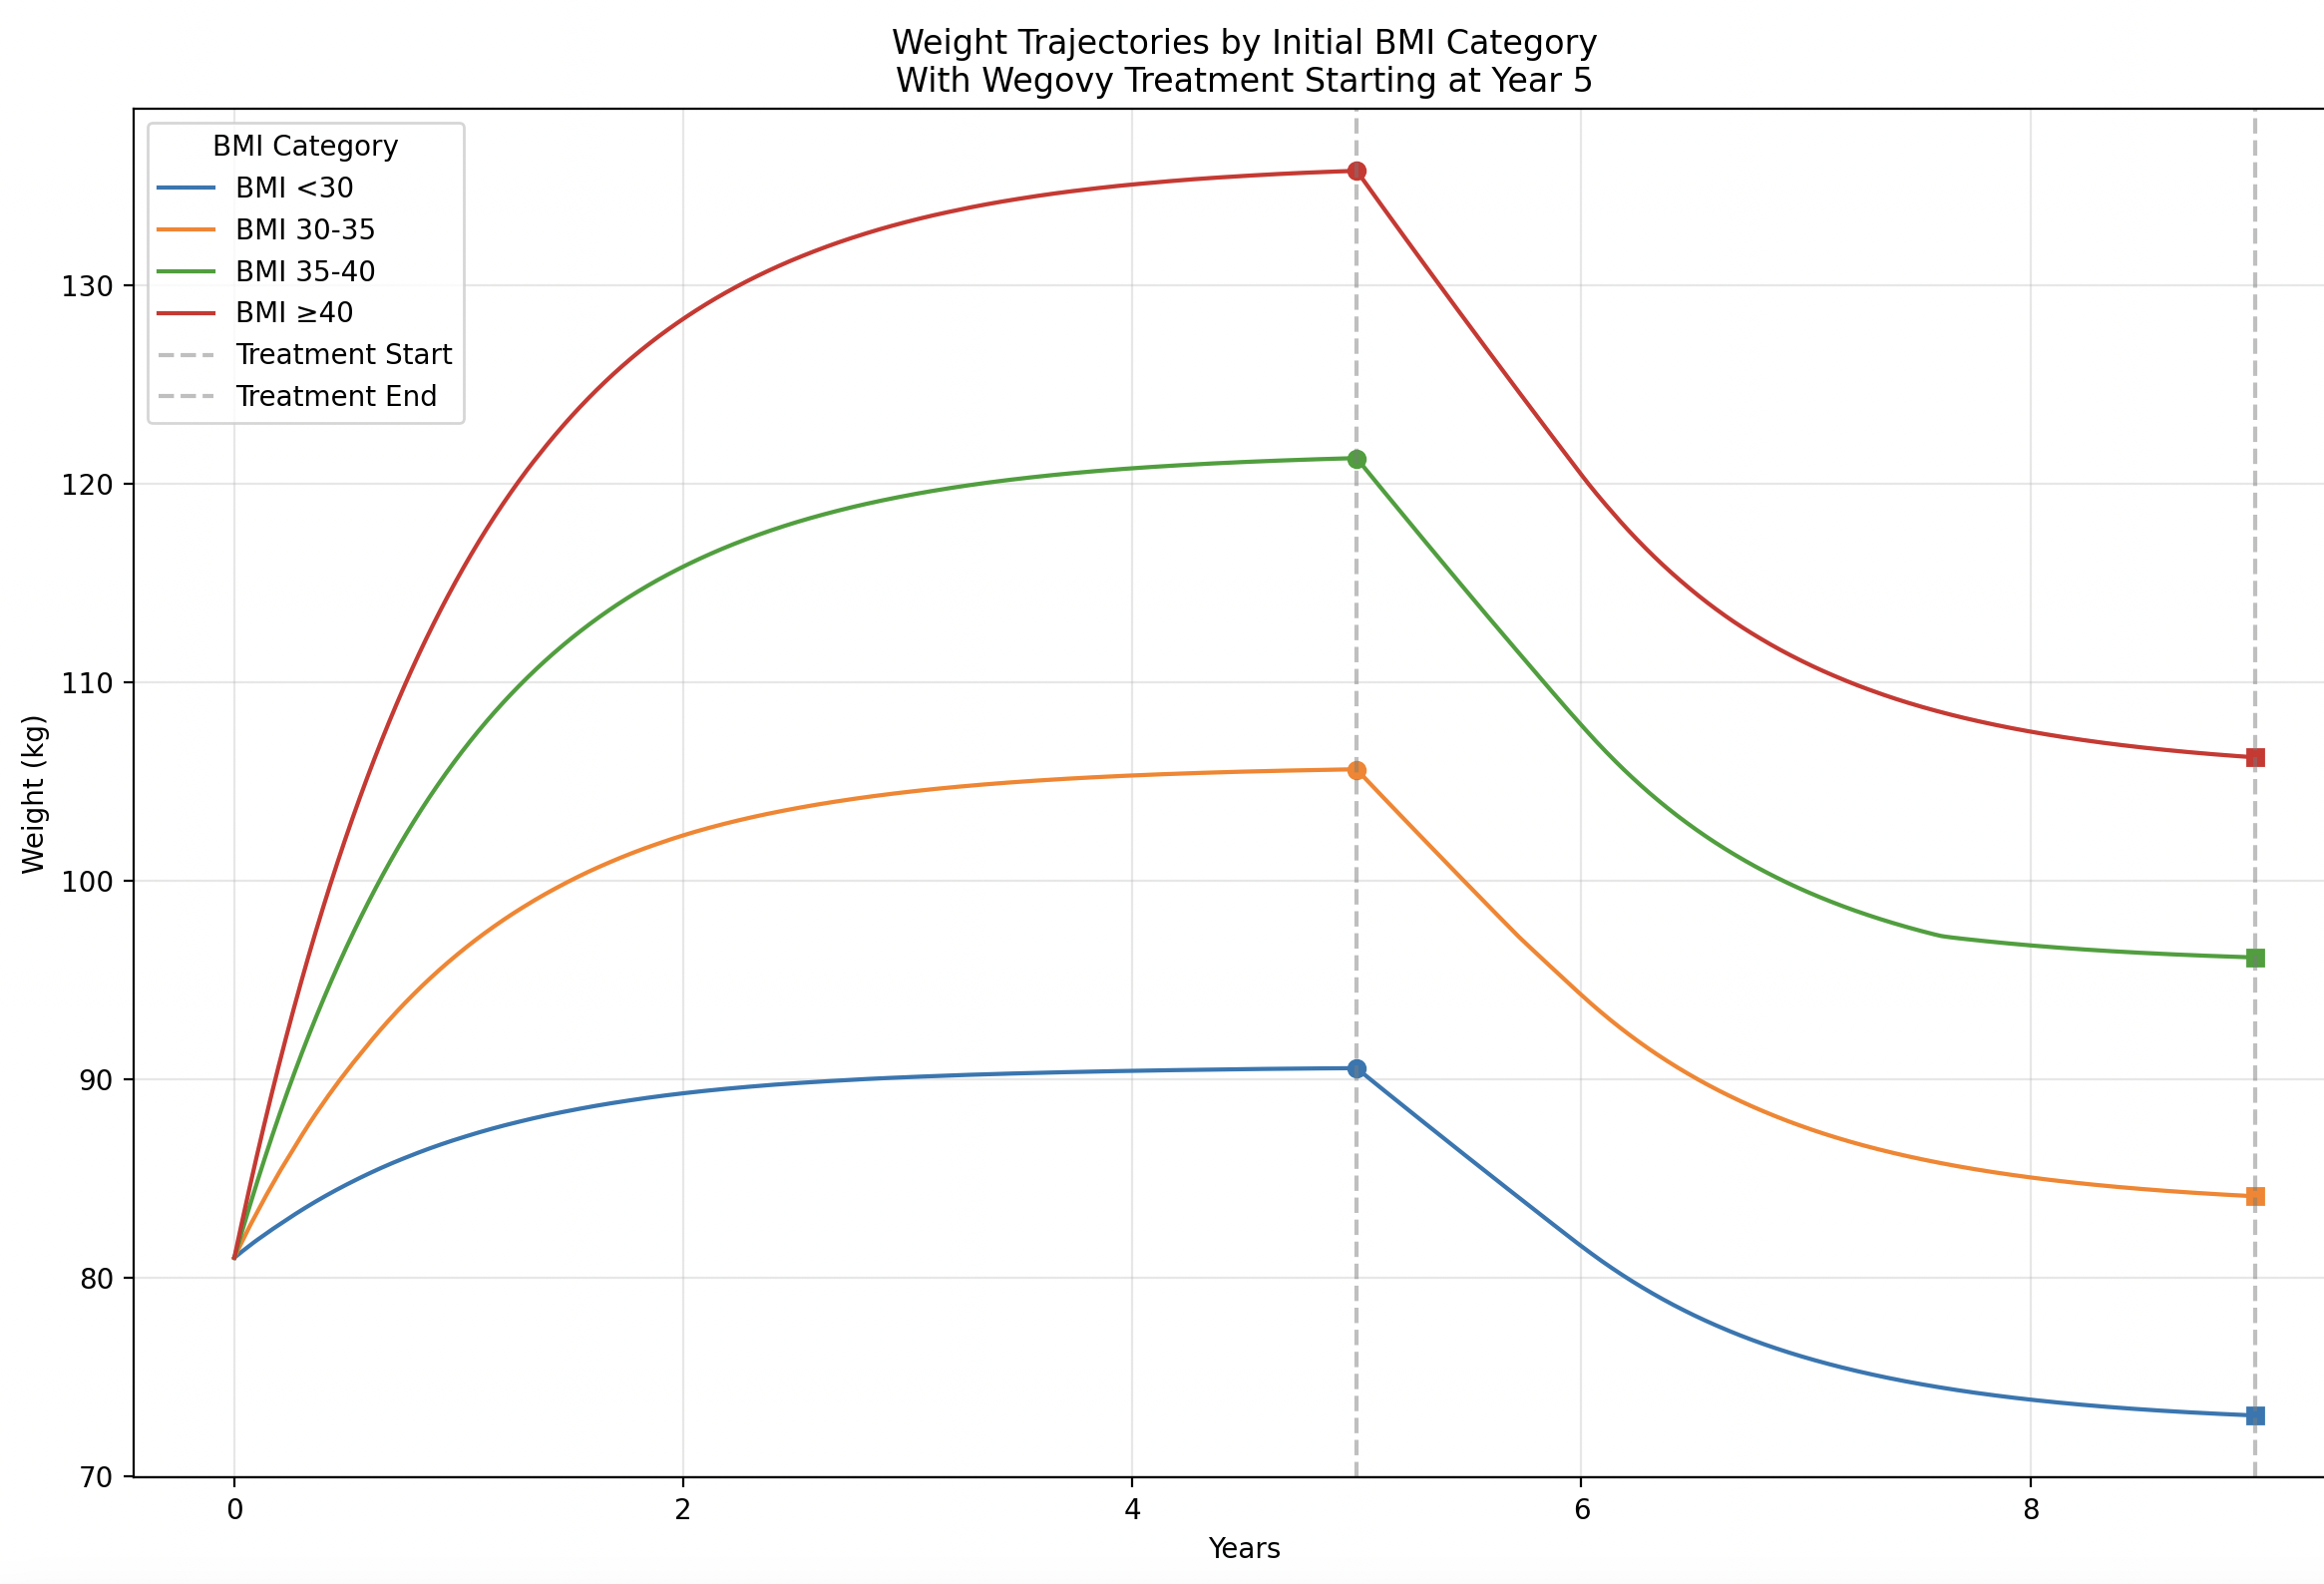
\includegraphics[width=0.8\textwidth]{images/wegovy_weights_plot.png}
\caption{Simulated weight trajectories by BMI category showing pre-treatment weight gain and subsequent Wegovy treatment response}
\label{fig:wegovy_weights}
\end{figure}

This matched the observed weight loss in the SELECT trial, indicating that our caloric requirements were accurate.

\subsection{Binary Search for Caloric Requirements}
To determine the caloric requirements for each phase of the trials, we implemented a binary search algorithm that finds the daily caloric intake needed to maintain a target weight. The algorithm:

\begin{enumerate}
    \item Sets an initial range of possible calories (1500-6000 kcal/day)
    \item Simulates weight trajectory for the midpoint caloric value
    \item Narrows the search range based on whether the final weight is above or below target
    \item Continues until the difference between final and target weight is within 0.1 kg
\end{enumerate}

This process yielded the following caloric requirements for the SELECT trial:

\begin{table}[h]
\centering
\begin{tabular}{|l|c|c|c|c|}
\hline
\textbf{BMI Group} & \textbf{Initial} & \textbf{Initial} & \textbf{Final} & \textbf{Final} \\
& \textbf{Weight (kg)} & \textbf{Calories} & \textbf{Weight (kg)} & \textbf{Calories} \\
\hline
BMI $<$30 & 76.2 & 2,353 & 68.2 & 2,098 \\
BMI 30-35 & 88.5 & 2,730 & 78.0 & 2,401 \\
BMI 35-40 & 102.1 & 3,152 & 89.8 & 2,766 \\
BMI $\geq$40 & 114.3 & 3,530 & 100.4 & 3,091 \\
\hline
\end{tabular}
\caption{Caloric requirements determined through binary search for SELECT trial phases}
\end{table}

And for the STEP trial:

\begin{table}[h]
\centering
\begin{tabular}{|l|c|c|c|c|}
\hline
\textbf{Initial BMI} & \textbf{Initial} & \textbf{Initial} & \textbf{Final} & \textbf{Final} \\
& \textbf{Weight (kg)} & \textbf{Calories} & \textbf{Weight (kg)} & \textbf{Calories} \\
\hline
38.6 & 105.1 & 3,245 & 88.2 & 2,634 \\
\hline
\end{tabular}
\caption{Caloric requirements determined through binary search for STEP trial phases}
\end{table}

\subsection{Model Parameter Adjustments}
Several parameters in our model were not directly measured in the clinical trials. To address this, we adjusted these parameters to match the observed biomarker values after two weeks of treatment. The following tables show the default values and the adjusted values for both trials:

\begin{table}[h]
\centering
\begin{tabular}{|l|c|c|c|c|}
\hline
\textbf{Parameter} & \textbf{Default} & \textbf{Post 2-Week} & \textbf{Units} \\
\hline
Free Fatty Acids & 400 & 688.65 & $\mu$mol/l \\
Insulin Sensitivity & 0.8 & 0.26 & ml/$\mu$U/day \\
Beta Cell Mass & 1009 & 1009 & mg \\
Insulin Secretion & 530 & 501.64 & $\mu$U/mg/day \\
Inflammation & 0.056 & 0.45 & dimensionless \\
\hline
\end{tabular}
\caption{Parameter adjustments for SELECT trial to match 2-week biomarkers}
\end{table}

\begin{table}[!h]
\centering
\begin{tabular}{|l|c|c|c|c|}
\hline
\textbf{Parameter} & \textbf{Default} & \textbf{Post 2-Week} & \textbf{Units} \\
\hline
Free Fatty Acids & 400 & 688.65 & $\mu$mol/l \\
Insulin Sensitivity & 0.8 & 0.26 & ml/$\mu$U/day \\
Beta Cell Mass & 1009 & 1009 & mg \\
Insulin Secretion & 530 & 501.64 & $\mu$U/mg/day \\
Inflammation & 0.056 & 0.45 & dimensionless \\
\hline
\end{tabular}
\caption{Parameter adjustments for STEP trial to match 2-week biomarkers}
\end{table}

These adjustments were essential for ensuring our model most accurately reflected the physiological changes observed in the clinical trials while maintaining consistency with known biological mechanisms.

\subsection{Creating the Ramp-Up Function}
To accurately model the gradual onset of Wegovy's appetite-suppressing effects, we implemented a ramp-up function that simulates the typical clinical titration schedule. The function gradually increases the medication's effect over time, which better reflects real-world patient experiences and helps avoid sudden caloric restrictions.

\begin{equation}
    \text{Ramp Factor} = \min\left(\frac{t - t_{\text{start}}}{t_{\text{ramp}}}, 1\right)
\end{equation}

where:
\begin{itemize}
    \item $t_{\text{start}}$ = 1825 days (5-year pre-treatment period)
    \item $t_{\text{ramp}}$ = 60 days (2-month ramp-up duration)
\end{itemize}

The caloric adjustment is then applied using:
\begin{equation}
    \text{Caloric Reduction} = \text{Target Reduction} \times \text{Ramp Factor}
\end{equation}

This gradual approach ensures that:
\begin{itemize}
    \item The treatment effect increases linearly over the first year
    \item The full effect is achieved only after complete titration
    \item The simulation better matches clinical observations of weight loss patterns
\end{itemize}


